
\subsection{Reference frame in SHADOW4}
\label{sec:reference_frame}


SHADOW use local reference systems associated to the source and image planes and to the beamline elements (see Fig.~\ref{fig:S4_reference_frame}).
This permits to iterate over the beamline elements: each one has two ``continuation planes": the source and the image. 

\begin{figure}[H]
\label{fig:S4_reference_frame}
    \centering
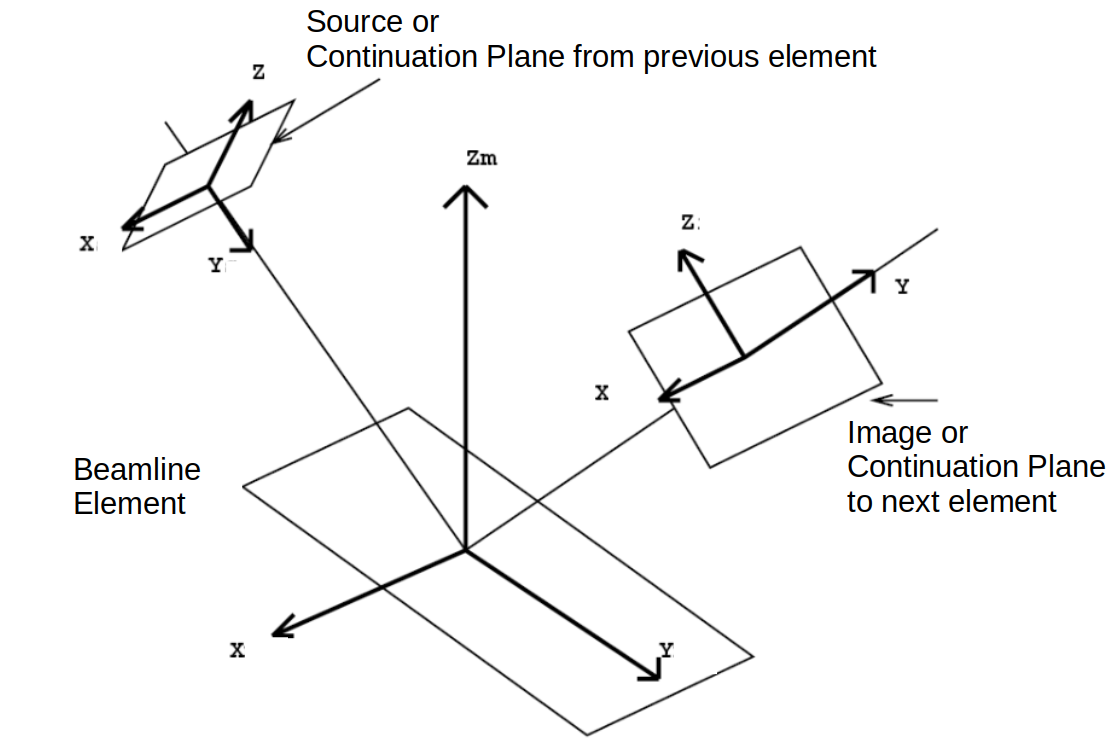
\includegraphics[width=0.9\linewidth]{reference-frames/S4_reference_frame.png}
\caption{SHADOW4 reference frame definitions: Source, beamline element, and image coordinates.}  
\end{figure}

In SHADOW4 the ``beamline element" is formed by an ``optical element" object and a ``coordinates" object containing two angles: the incidence angle $\theta$ and the beamline element orientation angle $\alpha$, and two distances: the distance $p$ from the source (or continuation plane from the previous element), and $q$ from the beamline element to its image plane or continuation plane.
The beamline element orientation angle $\alpha$ is not reset after the scattering in the beamline element (reflection, refraction or diffraction), therefore it influences the orientation of the axis at the image (see Fig.~\ref{fig:orientations}).

\begin{figure}
\label{fig:orientations}
    \centering
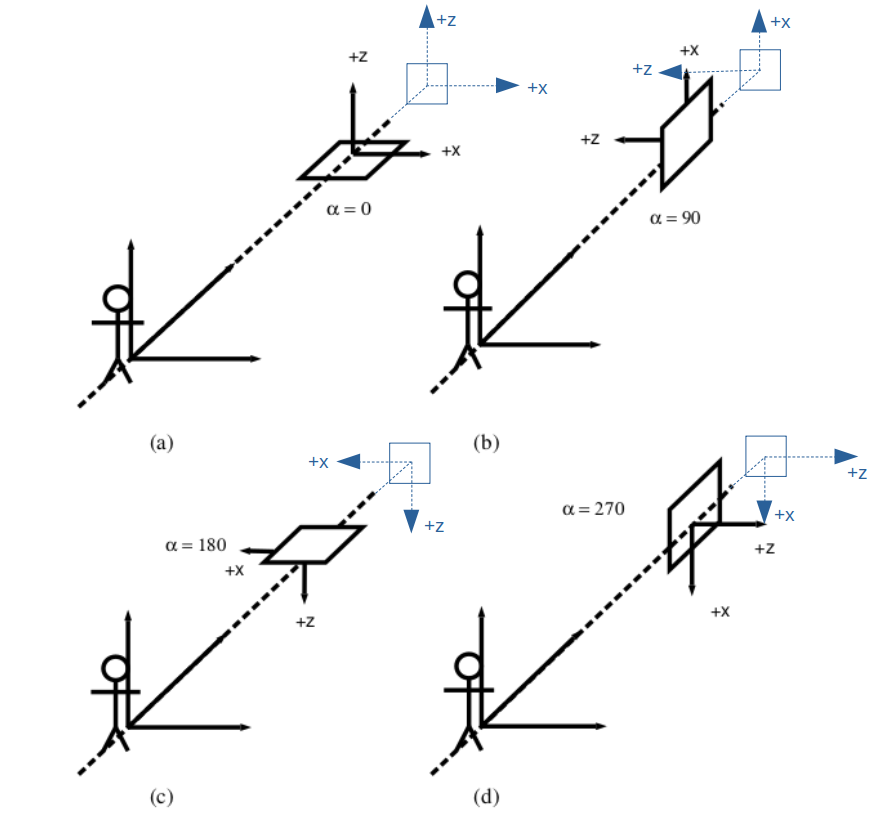
\includegraphics[width=0.9\linewidth]{reference-frames/S4_orientations.png}
\caption{Effect of the beamline element orientation angle $\alpha$ for the four most common values: 0, 90, 180 and 270 degrees. The effect of the angle $\alpha$ is carried out to the image plane, thus defining the position of the axes (in blue). }  
\end{figure}


